\documentclass[10pt,a4paper]{article}
\usepackage[T1]{fontenc}
\usepackage[scaled]{helvet}
\usepackage{cite}
\usepackage{url}
\usepackage{graphicx}
\usepackage{float}
\usepackage{amsmath}
\usepackage{amssymb}
\usepackage{fancyhdr}
\usepackage{lastpage}
\floatstyle{boxed} 
\restylefloat{figure}
\renewcommand*\familydefault{\sfdefault}
\title{Introduction to Operating Systems}
\author{David Lynch - david.lynch@raglansoftware.com }
\begin{document}
\maketitle
\begin{abstract}
In this article we step up from the physical hardware of the computer system and focus on the operating system, or where hardware meets software, meets the user. We take a look at the general structure of an operating system, some considerations when designing operating systems and define the roles and responsibilities of operating system software. There are a number of schools of thought on how operating systems should be designed and to illustrate the engineering problem, we look at a couple of approaches. 
\end{abstract}
\section{Introduction}
Formally, an operating system is a program that manages computer hardware. It provides a basis for application programs, such as word processors, by acting as an intermediary between the user and this hardware. Operating systems are found in wide ranges of computer driven devices. Each of these devices will have different important characteristics for which the operating system will be tailored. For example a main-frame controlled by OS 2200 Unisys will be engineered to cater for job execution and throughput, together with support for  multiple client users all managing the system. A personal computer system running Windows is tailored for user experience and responsiveness. An embedded real-time operating system such as LinuxOS RTOS is engineered to provide guarantees around how long computations will take. Lastly, a mobile operating system such as iOS6 will be optimized for user experience, power consumption and cater for various modes of interaction typically not supported by a personal computer.
\newline\newline
Each of the above examples can be examined in terms of the user or the system perspective. A microcomputer is designed for ease of use and responsiveness with little attention given to resource utilization, in contrast an embedded system is typically designed to run with little if any user interaction.
\begin{figure}
\caption{Abstract view of an operating system. \cite{OSCONCEPTS}}
\begin{center}
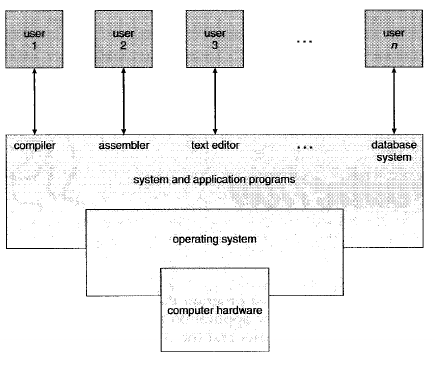
\includegraphics[scale=0.45]{../images/operating-system.png}
\label{os}
\end{center}
\end{figure}
\subsection{Structure}
A {\bf job} is defined as some unit of work to be executed by the computer system. In a single processor system with multiple jobs, only one job can access the system as once. In these systems {\bf multiprogramming} is used so that the CPU, as much as possible, has something to execute. It also facilitates {\bf multitasking} or {\bf time-sharing}, whereby multiple programs are {\bf switched} into and out of the CPU so that multiple programs and multiple users can be catered for. In the case where a user is interfacing with the computer system, it is said to be a {\bf response time sensitive} interaction. A program loaded into memory and either executing or ready for execution is called a {\bf process}. Processes that are {\bf I/O bound} will typically do a lot of waiting around for peripheral devices and are therefore good candidates for switching. In a typical scenario, a process that is waiting on an I/O operation to complete is switched out of the processor and a more CPU bound processes is switched in. A {\bf job pool} of switched out and processes is managed and maintained by the operating system. The decision making process is known as {\bf job scheduling} and is something we will consider in detail in this module. 
\newline\newline
The operating system must also assist in CPU scheduling. With multiple processes running at the same time, the operating system also needs to manage main memory and secondary storage, as well as I/O interactions with the user and tertiary devices. In doing this operating systems provide a means to {\bf allocate} and {\bf de-allocate} memory. Operating systems will also typically provide some form of {\bf virtual memory} that allows a process that is not completely in memory to be executed. A {\bf file system} is used to organise data that is to be kept on disk, which itself needs to be managed using a {\bf disk management} facility. Orderly execution of processes is guaranteed via job {\bf synchronization} and {\bf communication} mechanisms. 
\subsection{Interrupt Handling}
Modern Operating Systems are {\bf interrupt driven}. The CPU will react when it is interrupted by some event, such as an I/O request or a request to give up control of the CPU. A common interrupt is by the CPU timer, which will periodically interrupt the CPU. This can help ensure processes will give up the CPU for other process to use, particularly when instructed to do so. A {\bf trap} is a software generated interrupt. An {\bf interrupt handler} is a routine that exists for various type of interrupt and is responsible for reacting to the requested interrupt. An {\bf interrupt vector} stores the location in memory of the interrupt handler routine. A reserved area of memory typically known as the {\bf interrupt table} stores collections of these vectors. 
\subsection{Dual Mode Execution}
The operating system provides a means for the operations internally executed by the operating system is isolated from the effects of the program it is managing. This is commonly referred to as {\bf supervisor mode, kernel mode} or {\bf privileged mode}. {\bf Privileged Instructions} must execute in Kernel mode as they have the potential to influence the system as a whole. This protects the system from errant programmers and errant programmers from each other. The types of operations that should be executed in kernel mode are interrupt management, register management, some forms of memory management and I/O management. 
\begin{figure}
\caption{Separation of user and kernel space. \cite{OSCONCEPTS}}
\begin{center}
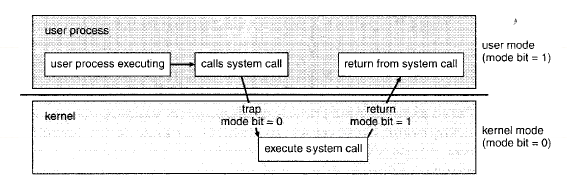
\includegraphics[scale=0.45]{../images/kernel-mode.png}
\label{kernelmode}
\end{center}
\end{figure}
\section{Process Management}
Any program in execution is a process. This is considered the unit of work in a computer system. Processes may also {\bf fork} {\bf sub-processes}. Processes require resources such as CPU, memory and files. A copy of the program counter is kept and associated with each process. Each program is executed in sequence for {\bf single threaded} processes, whereas {\bf multi-threaded} processes contain multiple program counters, which may be executed using some form of interleaved strategy. The operating system will also facilitate the following.
\begin{itemize}
\item Creation and Deletion of System and User Processes. 
\item Suspension and Resumption of a Process.
\item Process Synchronization.
\item Process Communication.
\item Handling of Deadlock.
\end{itemize}
\section{Memory Management}
For a program to be executed it must be mapped to an absolute address and loaded into main memory. The need to keep a program in memory, all with address translation and memory requirements, creates a need for memory management in its various guises. The memory management function keeps track of what parts of memory are currently being used by various processes. The allocation and deallocation of memory is a function whereby specific parts of memory are designated for use by one particular process. The contents of this memory must be protected when the process is switched out. The memory management function is also responsible for optimizing various performance characteristics of a system. Some mechanisms for this are discussed in later articles. 
\section{File Systems}
The OS provides a uniform logical view of information storage. The logical unit of storage is a {\bf file}. A file can be thought of as an abstraction of data on physical storage, essentially a collection of data defined by its creator. Files are organized into hierarchies called {\bf directories} for ease of use and organization. The operating system will implement one or more {\bf file systems} to assist in file management. Some examples of file systems are NTFS\cite{NTFS}, ZFS\cite{ZFS} and the Extended File System\cite{EXT}. We will not delve much more into file systems, however it is recommended you read up on the references of the previous three examples. 
\section{Storage Management}
Data that must endure beyond power down and data that will not fit in main memory must be save to secondary storage. The operating system is concerned with disk management, disk scheduling and the management of free space. This sub-system will guarantee the efficient use of secondary, and tertiary storage. {\bf Cache management} is closely related to storage management. As previously discussed, caches are vital to the performance of a system at various levels of the stack. Operating systems will manage their own caches, but not hardware related caches such as those we have discussed. Movement of data from main memory, which can be considered as a cache over secondary storage, can be looked upon as a caching problem. Therefore cache management and cache coherency is also a significant topic for operating systems. 
\section{I/O}
Operating systems must abstract away the peculiarities of dealing with particulars of different hardware with which the system communicates. The I/O sub-system is responsible for this. Functions supported by this sub system are buffering, caching, spooling as well as interaction with generic and hardware specific {\bf device drives}. We will not look at I/O in much detail but chapter 13 in \cite{OSCONCEPTS} is a highly recommended read that covers this complex topic in detail.
\section{Protection and Security}
With multiple users and concurrent execution of programs, access to data must be regulated by some means. {\bf Protection} is any mechanism for controlling access processes or users to the resource of a system. This facilitates protection from the corruption of data, from accessing data not suitable for access by some program and protection from rendering the system unusable. {\bf Security} is the mechanism whereby the system is protected from internal and external attacks. This includes attacks from viruses and unauthorized usage. We will look at these in much more detail in the Security module. Most operating systems will have a security model that encapsulates users, groups and privileges. Depending on which groups users are a member of, they will be granted specific privileges on the system. Protecting a system while still keeping protection overhead low is a tricky problem. Take a look at chapters 14 and 15 in \cite{OSCONCEPTS} for much more detail here. Consider this reference only reading. 
\section{Distributed Systems}
A distributed system is a collection of physically separate, possibly heterogeneous, computer systems that are networked to provide users with access to the various resources that the system as a whole maintains. A {\bf network} is simply the communication path between two or more systems. A large part of modern operating systems is responsible for managing and enabling communications across these networks. This includes various parts of the I/O services we mentioned previously, but also specific mechanisms such as implementation of the TCP/IP stack and Ethernet protocol. We will come back to Distributed Systems in a separate module. 
\section{OS Services}
Each of the functions above is facilitated by a {\bf service} provided by the operating system. Some categories of service are detailed below. 
\begin{itemize}
\item User Interface - Command Line or Graphical
\item Program Execution - Supporting the starting, termination and suspension of processing. 
\item I/O Subsystem - Providing a means to interact with devices.  
\item File System Manipulation - Creation, deletion and editing of files.
\item Communications - Between processes in the form of {\bf message passing} or {\bf shared memory}
\item Resource Allocation - Allocation of CPU and Memory
\item Accounting - Keeping track of usage of resources such as disk space. 
\item Protection and Security
\item Error Detection - Reporting and handling of CPU and I/O Errors. 
\end{itemize}
\section{System Calls}
Each of the above services of an operating system is typically exposed by one or more Application Program Interfaces, or API's. Most operating systems are written in lower level languages than Java. Typically, this means assembly, C, C++ and in practice a combination of all three. Two examples of standard API's are Microsoft's Win32-API \cite{WIN32API} and the POSIX standard API \cite{POSIXAPI}. \ref{systemcall} shows a simple system call. 
\begin{figure}
\caption{An example Win-32 system call. \cite{OSCONCEPTS}}
\begin{center}
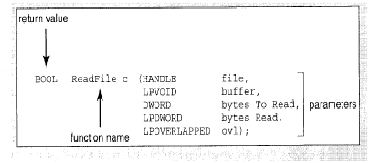
\includegraphics[scale=0.45]{../images/system-call.png}
\label{systemcall}
\end{center}
\end{figure}
The services shown in the previous section will each have an associated set of system calls. It is recommended here to read up on the POSIX standard API \cite{POSIXAPI}.
\section{The Kernel}
The Kernel is the core of the operating system and the actual bridge between applications and actual data processing by the hardware. A kernel can be thought of as the lowest layer of abstraction from the hardware. Different operating systems will have different types of services implemented at the kernel layer. Invariably, operating systems will ship with other software that compliment this kernel. For example, Windows Explorer is complimentary to file system set of system calls that are exposed by the Windows Kernel. More deeply, the common controls library, which is responsible for re-usable GUI controls is a complimentary library to the base kernel, and is re-used in most windows software. The distinction between the kernel layer and supporting software is malleable, although designs can be broadly classified into {\bf monolithic},{\bf micro}, which have different deliniations for which code is executed in kernel space, and {\bf hybrid} kernels where the lines become even more blurry. 
\subsection{Monolithic}
This approach to kernel design sees richly featured implementations of services such as schedulers, process managers and device drivers all contained within the kernel base and all running in kernel space. This facilitates efficient use of shared memory without the need of expensive IPC calls or kernel-to-user space switching. There are quite a few disadvantages to this approach however. There is high cohesion between implementation specific code such as device drivers and true base services such as schedulers. Over time, as large code bases such as kernels become highly cohesive, it becomes more difficult to develop and test upon them. Linux loadable kernel modules partially solve this problem. Linux is an example of a monolithic kernel. Windows XP is another example. 
\subsection{Micro}
An alternative approach to kernel design is to remove all non-essential code from the Kernel layer. What's left is typically basic inter-process communication and scheduling. The biggest distinction is that the supporting services such as application level IPC, device drivers and file servers are all run in user space. As a result, application processes never interact directly with the kernel. This design is arguably cleaner and more abstract and as a result easier to maintain. The penalty is typically framed as a performance hit. Each service will require at least one switch from user to kernel space to access underlying essential services. This requires a kernel to user space mode switch, to which a cost is associated. The Mach operating system kernel is an early example of a strict micro-kernel design. Figure \ref{monomicro} shows the distinction between the two approaches diagrammatically. 
\begin{figure}
\caption{Mono- vs. Micro- kernel design}
\begin{center}
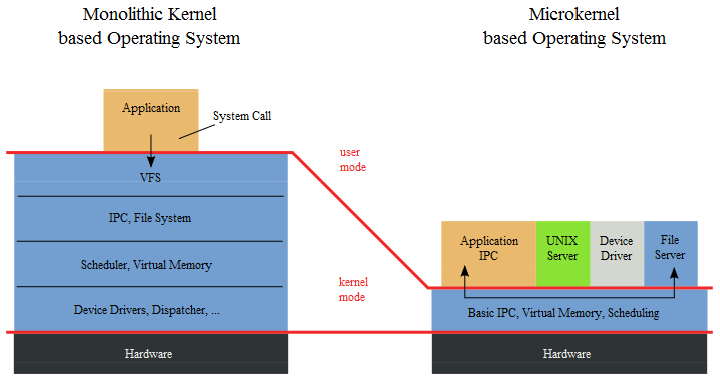
\includegraphics[scale=0.45]{../images/mono-vs-micro.png}
\label{monomicro}
\end{center}
\end{figure}
\subsection{Hybrid}
Mac OS X is an example of an operating system that uses elements of both approaches in a hybrid fashion. The Mach micro-kernel is used for core services such as memory management, IPC and RPC. To compliment this, the Berkeley Software Distribution, which is a UNIX operating system, is used to provide user command line interface, expose POSIX API's and provide thread libraries. Further complimenting this an I/O kit is implemented to support loadable kernel extensions and device drivers.  
\subsection{Further Reading}
There is a very interesting discussion conducted between Linus Torvalds and Andrew Tannenbaum on this, and other kernel level engineering problems here \cite{LINUSTANNEN}. Be sure to read the full version from this link as at the time of writing the Wikipedia article is quite poor. This is a good example of where pragmatism clearly won out over pure engineering.This will be a commonly running theme throughout your career - and expect to be paying off debts incurred by lazy programmers claming themselves to be pragmatists any time you work a on a code-base that is not 100% new! 
\subsection{Modules}
Modular techniques exist for most kernel architectures. A kernel will bootstrap with a core set of components and dynamically link in other modules at boot time. This allows the kernel to be customized to provide certain features dynamically. A set of protocols is defined around the implementation of these modules. Since kernel space is exposed by kernel modules, system designers must be careful about which kernel modules are integrated into the kernel. Anybody who has tried to compile and install a third party Linux kernel module will no doubt have some experience of the type of systems crashes that can be caused by poorly tested or implemented modules. This approach reflects loosely a layered system, although both monolithic and micro kernels can exhibit this feature. 
\section{Virtual Machines}
We introduce Virtual Machines here briefly as you will start using them quite soon to install Linux on your developer desktop. We will leave the full detail to another module on this course, but just outline it as a concept. In essence a virtual machine allows to abstract the hardware of a single computer onto several different environments. In doing so the illusion is created that each execution environment is running as its own computer. A virtualization layer provides the means to run concurrent {\bf guest} operating systems on some {\bf host} operating system. Figure \ref{virtualmachines} shows this in the abstract and figure \ref{vmarch} shows how the VMWare virtual machine works. Oracle Virtual Box \cite{VIRTUALBOX} is the VM of choice for this and other modules. We will run Linux as a guest operating system of Windows 7. This will be facilitated by the virtualization software and also facilitated by certain features of the x86 architecture \cite{INTELSWDEV}.
\begin{figure}
\caption{a) Non-Virtual and b) Virtual Machine \cite{OSCONCEPTS}}
\begin{center}
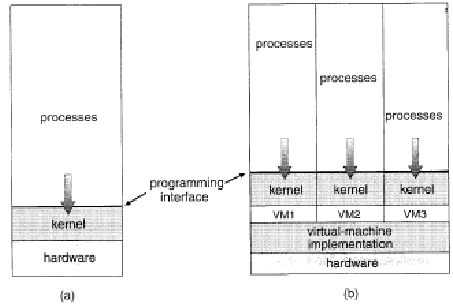
\includegraphics[scale=0.45]{../images/virtual-machine.png}
\label{virtualmachines}
\end{center}
\end{figure}
\begin{figure}
\caption{The VMWare Virtual Machine Architecture \cite{OSCONCEPTS}}
\begin{center}
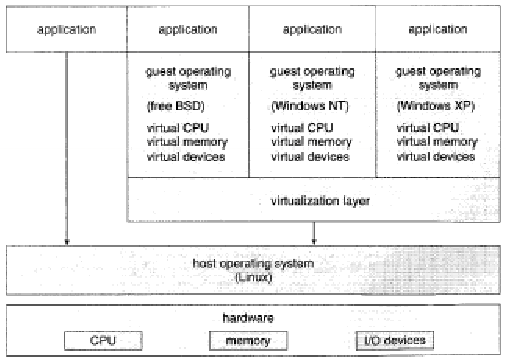
\includegraphics[scale=0.45]{../images/vm-arch.png}
\label{vmarch}
\end{center}
\end{figure}
\bibliography{../biblio/techfundamentals.bib}{}
\bibliographystyle{plain}
\begin{center}
\end{center}
\end{document}
